\subsection{Figure witnesses}\label{ex:fig-witnesses}
These schematic witnesses remain in the bip / biz / trit gauge. They illustrate the already-declared ledgers on the cited windows.

\paragraph{Figure F1: Q4 / two-cycle / four-cycle closure.}
\begin{center}
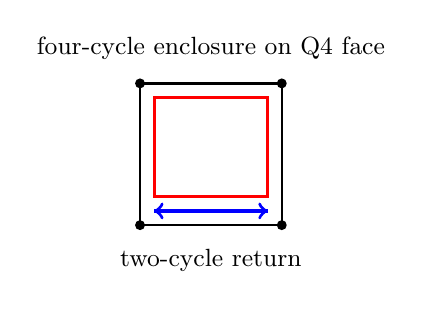
\begin{tikzpicture}[scale=0.9, every node/.style={font=\small}]
\coordinate (A) at (0,0); \coordinate (B) at (2,0); \coordinate (C) at (2,2); \coordinate (D) at (0,2);
\draw[thick] (A)--(B)--(C)--(D)--cycle;
\draw[very thick,blue,->] (0.2,0.2)--(1.8,0.2);
\draw[very thick,blue,->] (1.8,0.2)--(0.2,0.2);
\node at (1,-0.5) {two-cycle return};
\draw[very thick,red,->] (0.2,0.4)--(1.8,0.4)--(1.8,1.8)--(0.2,1.8)--cycle;
\node at (1,2.5) {four-cycle enclosure on Q4 face};
\fill (A) circle (2pt) (B) circle (2pt) (C) circle (2pt) (D) circle (2pt);
\end{tikzpicture}
\end{center}

\paragraph{Figure F2: $B^*$ ladder and attenuation.}
\begin{center}
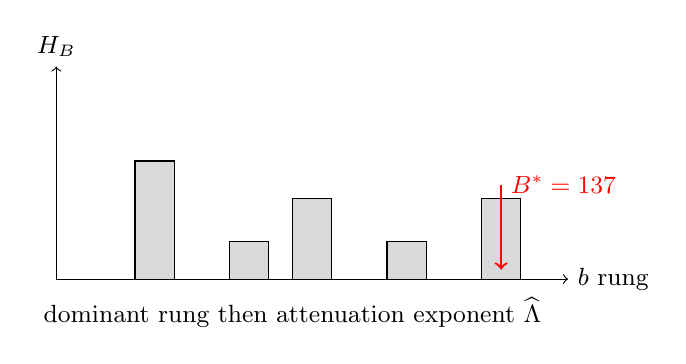
\begin{tikzpicture}[x=1cm,y=0.6cm, every node/.style={font=\small}]
\draw[->] (0,0) -- (6.5,0) node[right] {$b$ rung};
\draw[->] (0,0) -- (0,4.5) node[above] {$H_B$};
\draw[fill=gray!30] (1,0) rectangle +(0.5,2.5);
\draw[fill=gray!30] (2.2,0) rectangle +(0.5,0.8);
\draw[fill=gray!30] (3.0,0) rectangle +(0.5,1.7);
\draw[fill=gray!30] (4.2,0) rectangle +(0.5,0.8);
\draw[fill=gray!30] (5.4,0) rectangle +(0.5,1.7);
\draw[red,thick,->] (5.65,2) -- (5.65,0.2);
\node[red,right] at (5.65,2) {$B^*=137$};
\node at (3,-0.7) {dominant rung then attenuation exponent $\widehat\Lambda$};
\end{tikzpicture}
\end{center}

\paragraph{Figure F3: Collision / export-window diagram.}
\begin{center}
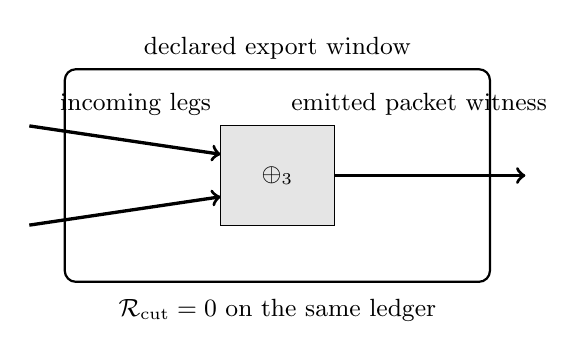
\begin{tikzpicture}[scale=0.9, every node/.style={font=\small}]
\draw[thick,rounded corners] (0,0) rectangle (6,3);
\node at (3,3.3) {declared export window};
\draw[->,very thick] (-0.5,2.2)--(2.2,1.8);
\draw[->,very thick] (-0.5,0.8)--(2.2,1.2);
\draw[fill=gray!20] (2.2,0.8) rectangle (3.8,2.2);
\node at (3,1.5) {$\oplus_3$};
\draw[->,very thick] (3.8,1.5)--(6.5,1.5);
\node at (1,2.5) {incoming legs};
\node at (5,2.5) {emitted packet witness};
\node at (3,-0.4) {$\mathcal R_{\mathrm{cut}}=0$ on the same ledger};
\end{tikzpicture}
\end{center}

\paragraph{Figure F4: Shell-band / cadence / torsion schematic.}
\begin{center}
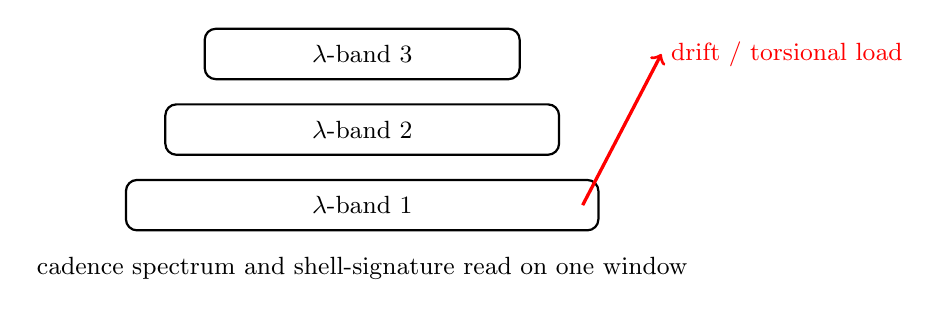
\begin{tikzpicture}[x=1cm,y=0.8cm, every node/.style={font=\small}]
\draw[thick,rounded corners] (0,0) rectangle (6,0.8);
\draw[thick,rounded corners] (0.5,1.2) rectangle (5.5,2);
\draw[thick,rounded corners] (1,2.4) rectangle (5,3.2);
\node at (3,0.4) {$\lambda$-band 1};
\node at (3,1.6) {$\lambda$-band 2};
\node at (3,2.8) {$\lambda$-band 3};
\draw[red,very thick,->] (5.8,0.4)--(6.8,2.8);
\node[red,right] at (6.8,2.8) {drift / torsional load};
\node at (3,-0.6) {cadence spectrum and shell-signature read on one window};
\end{tikzpicture}
\end{center}
